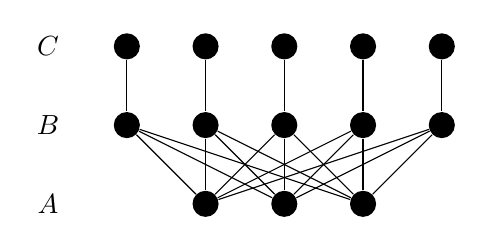
\begin{tikzpicture}
\foreach \x/\t in {2/A,1/B,0/C} {
  \node (T\x) at (0,-\x) {$\t$};
}
\foreach \x in {1,...,5} {
  \node[fill,circle] (A\x) at (\x,0) {};
  \node[fill,circle] (B\x) at (\x,-1) {};
  \draw (A\x) -- (B\x);
}
\foreach \x in {2,3,4} {
  \node[fill,circle] (C\x) at (\x,-2) {};
}
\foreach \x in {2,3,4} {
  \foreach \y in {1,...,5} {
    \draw (B\y) -- (C\x);
  }
}
\end{tikzpicture}